\documentclass[aspectratio=169, 11pt]{beamer}

% --- Packages & Setup ---
\usepackage[utf8]{inputenc}
\usepackage[T1]{fontenc}
\usepackage{helvet}
\renewcommand{\familydefault}{\sfdefault}
\usepackage{xcolor}
\usepackage{booktabs}
\usepackage{graphicx}
\usepackage{url}
\usepackage{tikz}
\usetikzlibrary{calc,arrows.meta,positioning,shapes.geometric}

\graphicspath{{../}{./}}

% --- Branding Colors ---
\definecolor{amritaMaroon}{HTML}{A4123F}
\definecolor{boxBg}{HTML}{F8F9FA}
\definecolor{borderGray}{HTML}{D1D5DB}
\definecolor{nodeBlue}{HTML}{E8F0FE}
\definecolor{accentGreen}{HTML}{0D9488}

% --- Theme Setup ---
\usetheme{Madrid}
\usecolortheme[named=amritaMaroon]{structure}
\setbeamertemplate{navigation symbols}{}
\setbeamertemplate{footline}[frame number]

\begin{document}

% =========================================================================
% SLIDE 1: TITLE SLIDE (Software-Based Project)
% =========================================================================
\begin{frame}
    % Corner Box Indicator
    \begin{tikzpicture}[remember picture,overlay]
        \node[fill=amritaMaroon, text=white, font=\bfseries\footnotesize, anchor=north east, rounded corners=2pt, inner sep=5pt]
        at ($(current page.north east) + (-0.2cm,-0.2cm)$)
        {Type 3: Software Project};
    \end{tikzpicture}

    \centering
    \includegraphics[width=2.6cm]{logo.png}
    \vspace{0.05cm}

    {\large \textbf{\textcolor{amritaMaroon}{M.A.C.H. AI: Multimodal Academic Cognitive Hub}}} \\
    {\small \textbf{A Fine-Tuned Graph-RAG Framework for Campus Knowledge Systems}} \\
    \vspace{0.05cm}
    {\footnotesize \textbf{23CSE498 -- Project Phase II (External Review)} \quad | \quad \textbf{Team Number: G081}} \\
    \vspace{0.10cm}

    % Student Table
    \begin{table}
        \centering
        \footnotesize
        \renewcommand{\arraystretch}{1.05}
        \begin{tabular}{|c|c|l|}
            \hline
            \textbf{S.No} & \textbf{Register Number} & \textbf{Student Name} \\
            \hline
            1 & CB.SC.U4CSE23505 & A. Chandra Vamsi \\
            \hline
            2 & CB.SC.U4CSE23508 & B. Prem Sai Charan \\
            \hline
            3 & CB.SC.U4CSE23530 & M. Pavan Prem Prabhas \\
            \hline
            4 & CB.SC.U4CSE23568 & P. Tirupati Reddy \\
            \hline
        \end{tabular}
    \end{table}
    \vspace{0.05cm}

    {\footnotesize Guide: \textbf{Dr. Shanmuga Priya S}, Assistant Professor (Sl.Gd.), Department of CSE} \\
    \vspace{0.05cm}
    {\scriptsize \today}
\end{frame}

% =========================================================================
% SLIDE 2: GUIDE APPROVAL EMAIL CONFIRMATION (Mandatory)
% =========================================================================
\begin{frame}{Guide Review \& Submission Approval}
    \framesubtitle{Confirmation of Project Review and Approval from Guide}
    \centering
    \fbox{\begin{minipage}[c][5.2cm]{0.94\textwidth}
        \centering
        \textbf{[Insert Screenshot of Guide Approval Email Here]} \\[0.3cm]
        {\footnotesize [Mandatory: Attach a clear, readable screenshot of the email received from Dr. Shanmuga Priya S approving this presentation and final review submission]}
    \end{minipage}}
\end{frame}

% =========================================================================
% SECTION 1: PROBLEM DEFINITION, MOTIVATION & SOLUTION DESIGN (5 MARKS)
% =========================================================================
\section{Problem Definition \& Solution Design}

% --- SLIDE 3: PROBLEM DEFINITION & MOTIVATION ---
\begin{frame}{1. Problem Definition \& Motivation}
    \framesubtitle{Challenges in Academic Campus Knowledge Discovery}
    \begin{columns}[T]
        \column{0.48\textwidth}
        \begin{block}{Existing Limitations \& Pain Points}
            \footnotesize
            \begin{itemize}
                \item \textbf{Curriculum Data Silos:} Syllabi, regulations, exam seating, and past question papers are scattered across PDFs with inconsistent formatting.
                \item \textbf{Naive Vector RAG Failures:} Standard chunking loses hierarchical course relationships (Course $\rightarrow$ Unit $\rightarrow$ Topic $\rightarrow$ Prerequisite), causing hallucinations.
                \item \textbf{Cloud Privacy Risks:} Sending internal student and exam records to commercial cloud LLMs violates institutional data privacy.
            \end{itemize}
        \end{block}

        \column{0.48\textwidth}
        \begin{block}{Our Proposed Solution: M.A.C.H. AI}
            \footnotesize
            \begin{itemize}
                \item \textbf{Hybrid Graph-RAG Architecture:} Combines Neo4j property graphs for deterministic syllabus traversal with pgvector for semantic retrieval.
                \item \textbf{100\% On-Premise Execution:} Air-gapped deployment with local quantized LLM (\texttt{gemma4:12b-it-qat}) and local embeddings.
                \item \textbf{Multimodal PYQ Discovery:} Automated bounding-box cropping for circuit diagrams and math formulas rendered via KaTeX.
            \end{itemize}
        \end{block}
    \end{columns}
    \vspace{0.15cm}
    \begin{alertblock}{Design Objective}
        \scriptsize
        Build a production-ready, sub-second academic hub that answers curriculum questions deterministically without LLM overhead, while serving multimodal past paper questions with high precision.
    \end{alertblock}
\end{frame}

% --- SLIDE 4: SOFTWARE REQUIREMENTS SPECIFICATION (SRS) ---
\begin{frame}{2. Software Requirements Specification (SRS)}
    \framesubtitle{Primary Actors, Core Functional \& Non-Functional Requirements}
    \begin{columns}[T]
        \column{0.48\textwidth}
        \begin{block}{Primary Actors \& Scope}
            \footnotesize
            \begin{itemize}
                \item \textbf{Student:} Queries course prerequisites, syllabus units, exam questions filtered by topic, and seating allocations.
                \item \textbf{Administrator:} Uploads academic documents, synchronizes the Neo4j graph, and inspects system health.
            \end{itemize}
        \end{block}

        \begin{block}{Non-Functional Requirements (NFR)}
            \footnotesize
            \begin{itemize}
                \item \textbf{[NFR-01] Latency:} Fast-path graph lookups $<50$\,ms; time-to-first-token (TTFT) $<450$\,ms.
                \item \textbf{[NFR-02] Privacy:} 100\% local execution, zero external data leakage, JWT RBAC security.
                \item \textbf{[NFR-03] Memory Efficiency:} Half-precision embeddings (\texttt{halfvec}) saving 50\% RAM.
            \end{itemize}
        \end{block}

        \column{0.48\textwidth}
        \begin{block}{Functional Requirements (FR)}
            \footnotesize
            \begin{itemize}
                \item \textbf{[FR-01] Fast-Path Curriculum Traversal:} Deterministic Neo4j retrieval of course units and prerequisites bypassing LLM inference.
                \item \textbf{[FR-02] Hybrid Multimodal Retrieval:} Reciprocal Rank Fusion (RRF) combining dense \texttt{halfvec(768)} and sparse BM25 keyword matching.
                \item \textbf{[FR-03] Contrastive Topic Isolation:} Explicit negative keyword filtering preventing topic leakage (e.g., capacitors vs. resistors).
                \item \textbf{[FR-04] Document QA \& Cropper:} Structured extraction of seating and calendar data; automatic circuit diagram cropping from PDFs.
            \end{itemize}
        \end{block}
    \end{columns}
\end{frame}

% --- SLIDE 5: SOFTWARE SYSTEM ARCHITECTURE (FULL-WIDTH 4 TIERS) ---
\begin{frame}{3. Software System Architecture}
    \framesubtitle{Frontend Tier $\longleftrightarrow$ API / Service Layer $\longleftrightarrow$ Business Logic $\longleftrightarrow$ Database / Storage Tier}
    \centering
    \resizebox{0.96\linewidth}{!}{
        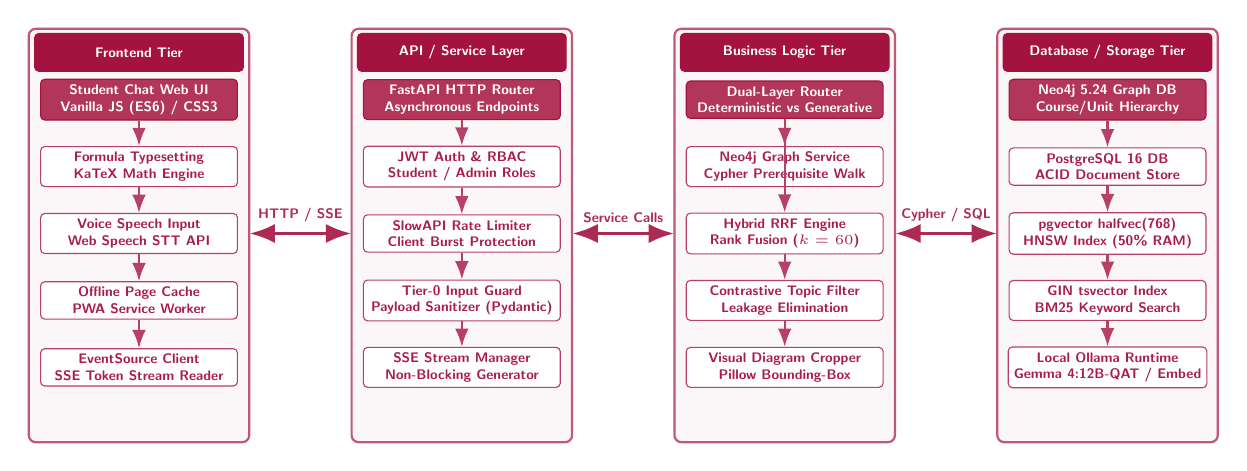
\begin{tikzpicture}[
            font=\tiny,
            tierbox/.style={draw=amritaMaroon!70, fill=amritaMaroon!4, rounded corners=2.5pt, thick},
            tierhdr/.style={draw=amritaMaroon, fill=amritaMaroon, text=white, rounded corners=1.5pt,
                            minimum width=2.65cm, minimum height=0.48cm, align=center, font=\tiny\bfseries, inner sep=2pt},
            subnode/.style={draw=amritaMaroon!80, fill=white, text=amritaMaroon!95, rounded corners=1.5pt,
                            minimum width=2.5cm, minimum height=0.44cm, align=center, font=\tiny\bfseries, inner sep=2pt},
            subnodeDark/.style={draw=amritaMaroon, fill=amritaMaroon!85, text=white, rounded corners=1.5pt,
                                minimum width=2.5cm, minimum height=0.44cm, align=center, font=\tiny\bfseries, inner sep=2pt},
            arr/.style={->, >=Latex, thick, color=amritaMaroon!80},
            tierArr/.style={<->, >=Latex, line width=1.4pt, color=amritaMaroon!90}
        ]

            %% ==========================================
            %% 1. FRONTEND TIER
            %% ==========================================
            \draw[tierbox] (-1.4, -4.1) rectangle (1.4, 1.15);
            \node[tierhdr] at (0, 0.85) {Frontend Tier};
            \node[subnodeDark] (fe1) at (0,  0.25) {Student Chat Web UI\\Vanilla JS (ES6) / CSS3};
            \node[subnode]     (fe2) at (0, -0.60) {Formula Typesetting\\KaTeX Math Engine};
            \node[subnode]     (fe3) at (0, -1.45) {Voice Speech Input\\Web Speech STT API};
            \node[subnode]     (fe4) at (0, -2.30) {Offline Page Cache\\PWA Service Worker};
            \node[subnode]     (fe5) at (0, -3.15) {EventSource Client\\SSE Token Stream Reader};
            \draw[arr](fe1)--(fe2); \draw[arr](fe2)--(fe3);
            \draw[arr](fe3)--(fe4); \draw[arr](fe4)--(fe5);

            %% ==========================================
            %% 2. API / SERVICE LAYER
            %% ==========================================
            \draw[tierbox] (2.7, -4.1) rectangle (5.5, 1.15);
            \node[tierhdr] at (4.1, 0.85) {API / Service Layer};
            \node[subnodeDark] (ap1) at (4.1,  0.25) {FastAPI HTTP Router\\Asynchronous Endpoints};
            \node[subnode]     (ap2) at (4.1, -0.60) {JWT Auth \& RBAC\\Student / Admin Roles};
            \node[subnode]     (ap3) at (4.1, -1.45) {SlowAPI Rate Limiter\\Client Burst Protection};
            \node[subnode]     (ap4) at (4.1, -2.30) {Tier-0 Input Guard\\Payload Sanitizer (Pydantic)};
            \node[subnode]     (ap5) at (4.1, -3.15) {SSE Stream Manager\\Non-Blocking Generator};
            \draw[arr](ap1)--(ap2); \draw[arr](ap2)--(ap3);
            \draw[arr](ap3)--(ap4); \draw[arr](ap4)--(ap5);

            %% ==========================================
            %% 3. BUSINESS LOGIC TIER
            %% ==========================================
            \draw[tierbox] (6.8, -4.1) rectangle (9.6, 1.15);
            \node[tierhdr] at (8.2, 0.85) {Business Logic Tier};
            \node[subnodeDark] (bl1) at (8.2,  0.25) {Dual-Layer Router\\Deterministic vs Generative};
            \node[subnode]     (bl2) at (8.2, -0.60) {Neo4j Graph Service\\Cypher Prerequisite Walk};
            \node[subnode]     (bl3) at (8.2, -1.45) {Hybrid RRF Engine\\Rank Fusion ($k=60$)};
            \node[subnode]     (bl4) at (8.2, -2.30) {Contrastive Topic Filter\\Leakage Elimination};
            \node[subnode]     (bl5) at (8.2, -3.15) {Visual Diagram Cropper\\Pillow Bounding-Box};
            \draw[arr](bl1)--(bl2); \draw[arr](bl1)--(bl3);
            \draw[arr](bl3)--(bl4); \draw[arr](bl4)--(bl5);

            %% ==========================================
            %% 4. DATABASE / STORAGE TIER
            %% ==========================================
            \draw[tierbox] (10.9, -4.1) rectangle (13.7, 1.15);
            \node[tierhdr] at (12.3, 0.85) {Database / Storage Tier};
            \node[subnodeDark] (db1) at (12.3,  0.25) {Neo4j 5.24 Graph DB\\Course/Unit Hierarchy};
            \node[subnode]     (db2) at (12.3, -0.60) {PostgreSQL 16 DB\\ACID Document Store};
            \node[subnode]     (db3) at (12.3, -1.45) {pgvector halfvec(768)\\HNSW Index (50\% RAM)};
            \node[subnode]     (db4) at (12.3, -2.30) {GIN tsvector Index\\BM25 Keyword Search};
            \node[subnode]     (db5) at (12.3, -3.15) {Local Ollama Runtime\\Gemma 4:12B-QAT / Embed};
            \draw[arr](db1)--(db2); \draw[arr](db2)--(db3);
            \draw[arr](db3)--(db4); \draw[arr](db4)--(db5);

            %% ==========================================
            %% INTER-TIER CONNECTIONS (<->)
            %% ==========================================
            \draw[tierArr] (1.4, -1.45) -- node[above, font=\tiny\bfseries, text=amritaMaroon!90] {HTTP / SSE} (2.7, -1.45);
            \draw[tierArr] (5.5, -1.45) -- node[above, font=\tiny\bfseries, text=amritaMaroon!90] {Service Calls} (6.8, -1.45);
            \draw[tierArr] (9.6, -1.45) -- node[above, font=\tiny\bfseries, text=amritaMaroon!90] {Cypher / SQL} (10.9, -1.45);

        \end{tikzpicture}
    }
    \vspace{0.10cm}
    \begin{block}{Architectural Overview}
        \scriptsize
        Decoupled 4-tier architecture: The Frontend Tier communicates via REST and SSE with the API / Service Layer. The Business Logic Tier executes deterministic queries directly on Neo4j ($<50$\,ms) and routes conceptual inquiries through Hybrid RRF into the Database / Storage Tier and local Ollama inference engine.
    \end{block}
\end{frame}

% --- SLIDE 6: MODULE BREAKDOWN ---
\begin{frame}{4. Module Breakdown \& Subsystem Architecture}
    \framesubtitle{Decomposition of Presentation, Gateway, Processing \& Data Layers}
    \begin{itemize}
        \item \textbf{Web Frontend Client:} Standards-compliant UI for document management and real-time interaction via Server-Sent Events (SSE) token streaming. Renders mathematical formulas client-side with KaTeX and supports voice input via Web Speech API.
        \item \textbf{API Gateway (FastAPI):} Asynchronous entry point managing REST endpoints, JWT role-based access control, SlowAPI rate limiting, and asynchronous background task queuing.
        \item \textbf{Processing \& Retrieval Engine:}
        \begin{itemize}
            \item \textit{PDF Parser \& Cropper:} Extracts hierarchical text from syllabi and dynamically crops question boundaries and diagrams using PyMuPDF and Pillow.
            \item \textit{Hybrid Retrieval Module:} Implements Reciprocal Rank Fusion (RRF, $k=60$) combining dense semantic vectors (\texttt{halfvec(768)}) with sparse BM25 keyword matching.
            \item \textit{Knowledge Graph Constructor:} Builds structural curriculum graphs linking Courses, Units, and Topics in Neo4j.
        \end{itemize}
        \item \textbf{Data Layer:} Polyglot persistence architecture combining PostgreSQL 16 (\texttt{pgvector}) for chunks and question metadata with Neo4j 5.24 for hierarchical graph traversals.
    \end{itemize}
\end{frame}

% --- SLIDE 7: CORE API SPECIFICATIONS ---
\begin{frame}{5. Core API Specifications}
    \framesubtitle{REST and Streaming Interface Contracts Across System Boundaries}
    \begin{itemize}
        \item \textbf{\texttt{POST /api/academic/upload}}
        \begin{itemize}
            \item \textit{Inputs:} \texttt{multipart/form-data} (PDF file, \texttt{course\_code}, \texttt{doc\_type}: \texttt{syllabus} | \texttt{pyq}).
            \item \textit{Function:} Persists file metadata, initiates transaction, and dispatches non-blocking async background extraction.
        \end{itemize}
        \item \textbf{\texttt{POST /api/chat/stream}}
        \begin{itemize}
            \item \textit{Inputs:} JSON (\texttt{message}, \texttt{session\_id}, \texttt{course\_code}).
            \item \textit{Function:} Routes query through intent classifier, executes fast-path Neo4j lookup or hybrid RRF, and streams answer tokens via SSE.
        \end{itemize}
        \item \textbf{\texttt{GET /api/documents}}
        \begin{itemize}
            \item \textit{Function:} Fetches tracking status (\texttt{pending}, \texttt{processing}, \texttt{completed}, \texttt{failed}) of ingested files.
        \end{itemize}
        \item \textbf{\texttt{GET /api/pyq/crop/\{id\}}}
        \begin{itemize}
            \item \textit{Function:} Returns binary PNG of auto-cropped circuit schematics and math diagrams for inline rendering.
        \end{itemize}
    \end{itemize}
\end{frame}

% --- SLIDE 8: UML DIAGRAM 1: FILE UPLOAD PROCESS ---
\begin{frame}{6. UML Sequence: File Upload \& Ingestion Process}
  \framesubtitle{Asynchronous ingestion with conditional branching for Curriculum vs. PYQ}
  \vspace{-0.3cm}
  \centering
  \resizebox{!}{0.76\textheight}{%
  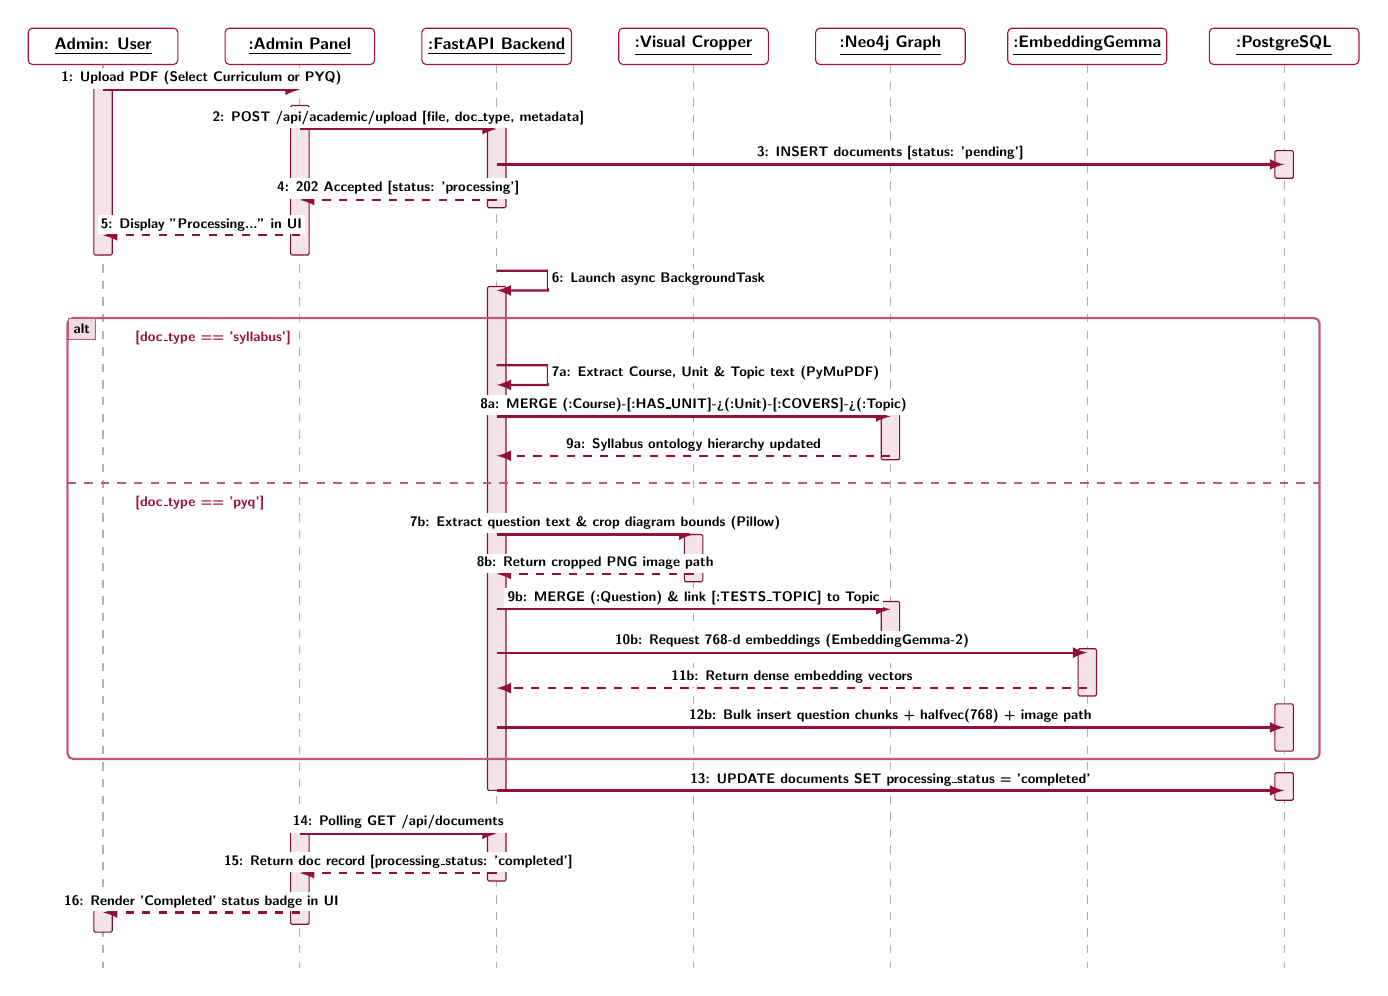
\begin{tikzpicture}[
    font=\scriptsize,
    >=latex,
    umllbl/.style={font=\fontsize{5.4pt}{6.4pt}\selectfont\bfseries, text=black, fill=white, inner sep=1.2pt},
    umlpart/.style={draw=amritaMaroon, fill=white, text=black, rounded corners=1.5pt, minimum width=1.9cm, minimum height=0.46cm, align=center, font=\fontsize{6.2pt}{7.2pt}\selectfont\bfseries, inner sep=2pt},
    umlact/.style={draw=amritaMaroon!80!black, fill=amritaMaroon!12, rounded corners=0.5pt, minimum width=0.22cm},
    umlmsg/.style={->, thick, draw=amritaMaroon!90!black},
    umlret/.style={->, thick, dashed, draw=amritaMaroon!90!black},
    altbox/.style={draw=amritaMaroon!70, thick, rounded corners=2pt},
    altguard/.style={font=\fontsize{5.5pt}{6.5pt}\selectfont\bfseries, text=amritaMaroon!95!black, fill=white, inner sep=1.5pt}
  ]
    % --- 7 Lifeline Participants (spaced at 2.5cm) ---
    \node[umlpart] (a)   at (0.0,   0.0) {\underline{Admin: User}};
    \node[umlpart] (fe)  at (2.5,   0.0) {\underline{:Admin Panel}};
    \node[umlpart] (be)  at (5.0,   0.0) {\underline{:FastAPI Backend}};
    \node[umlpart] (crp) at (7.5,   0.0) {\underline{:Visual Cropper}};
    \node[umlpart] (neo) at (10.0,  0.0) {\underline{:Neo4j Graph}};
    \node[umlpart] (olm) at (12.5,  0.0) {\underline{:EmbeddingGemma}};
    \node[umlpart] (pg)  at (15.0,  0.0) {\underline{:PostgreSQL}};

    % --- Vertical Dashed Lifelines ---
    \draw[dashed, gray!60] (a)   -- ++(0, -11.7);
    \draw[dashed, gray!60] (fe)  -- ++(0, -11.7);
    \draw[dashed, gray!60] (be)  -- ++(0, -11.7);
    \draw[dashed, gray!60] (crp) -- ++(0, -11.7);
    \draw[dashed, gray!60] (neo) -- ++(0, -11.7);
    \draw[dashed, gray!60] (olm) -- ++(0, -11.7);
    \draw[dashed, gray!60] (pg)  -- ++(0, -11.7);

    % --- Activation Bars (Execution Specifications) ---
    \node[umlact, minimum height=2.3cm] at (0.0,  -1.50) {};
    \node[umlact, minimum height=1.9cm] at (2.5,  -1.70) {};
    \node[umlact, minimum height=1.1cm] at (5.0,  -1.50) {};
    \node[umlact, minimum height=0.35cm] at (15.0,-1.50) {};

    % Background Worker Activation on Backend
    \node[umlact, minimum height=6.4cm] at (5.0,  -6.25) {};
    \node[umlact, minimum height=0.6cm] at (10.0, -4.95) {};
    \node[umlact, minimum height=0.6cm] at (7.5,  -6.50) {};
    \node[umlact, minimum height=0.6cm] at (10.0, -7.35) {};
    \node[umlact, minimum height=0.6cm] at (12.5, -7.95) {};
    \node[umlact, minimum height=0.6cm] at (15.0, -8.65) {};

    % Phase 3 Activation
    \node[umlact, minimum height=0.35cm] at (15.0,-9.40) {};
    \node[umlact, minimum height=1.3cm] at (2.5,  -10.50) {};
    \node[umlact, minimum height=0.7cm] at (5.0,  -10.25) {};
    \node[umlact, minimum height=0.5cm] at (0.0,  -11.00) {};

    % =========================================================================
    % PHASE 1: Non-Blocking Submission & Immediate Response
    % =========================================================================
    \draw[umlmsg] (0.0, -0.55) -- node[above, umllbl] {1: Upload PDF (Select Curriculum or PYQ)} (2.5, -0.55);
    \draw[umlmsg] (2.5, -1.05) -- node[above, umllbl] {2: POST /api/academic/upload [file, doc\_type, metadata]} (5.0, -1.05);
    \draw[umlmsg] (5.0, -1.50) -- node[above, umllbl] {3: INSERT documents [status: 'pending']} (15.0, -1.50);
    \draw[umlret] (5.0, -1.95) -- node[above, umllbl] {4: 202 Accepted [status: 'processing']} (2.5, -1.95);
    \draw[umlret] (2.5, -2.40) -- node[above, umllbl] {5: Display "Processing..." in UI} (0.0, -2.40);

    % Kickoff async task
    \draw[umlmsg] (5.0, -2.85) -- ++(0.65,0) -- ++(0,-0.25) -- (5.0,-3.10);
    \node[umllbl, anchor=west] at (5.65, -2.95) {6: Launch async BackgroundTask};

    % =========================================================================
    % PHASE 2: UML 'alt' Combined Fragment (Conditional Pipeline)
    % =========================================================================
    \draw[altbox] (-0.45, -3.45) rectangle (15.45, -9.05);
    \node[draw=amritaMaroon!70, fill=amritaMaroon!15, font=\fontsize{5.5pt}{6.5pt}\selectfont\bfseries, inner sep=2pt, anchor=north west] 
      at (-0.45, -3.45) {alt};

    % --- Branch 1: Curriculum / Syllabus ---
    \node[altguard, anchor=west] at (0.35, -3.70) {[doc\_type == 'syllabus']};

    \draw[umlmsg] (5.0, -4.05) -- ++(0.65,0) -- ++(0,-0.25) -- (5.0,-4.30);
    \node[umllbl, anchor=west] at (5.65, -4.15) {7a: Extract Course, Unit \& Topic text (PyMuPDF)};

    \draw[umlmsg] (5.0, -4.70) -- node[above, umllbl] {8a: MERGE (:Course)-[:HAS\_UNIT]->(:Unit)-[:COVERS]->(:Topic)} (10.0, -4.70);
    \draw[umlret] (10.0,-5.20) -- node[above, umllbl] {9a: Syllabus ontology hierarchy updated} (5.0, -5.20);

    % --- Dashed Separator Line for Alternative Branch ---
    \draw[dashed, thick, amritaMaroon!70] (-0.45, -5.55) -- (15.45, -5.55);

    % --- Branch 2: Previous Year Question Paper (PYQ) ---
    \node[altguard, anchor=west] at (0.35, -5.80) {[doc\_type == 'pyq']};

    \draw[umlmsg] (5.0, -6.20) -- node[above, umllbl] {7b: Extract question text \& crop diagram bounds (Pillow)} (7.5, -6.20);
    \draw[umlret] (7.5, -6.70) -- node[above, umllbl] {8b: Return cropped PNG image path} (5.0, -6.70);

    \draw[umlmsg] (5.0, -7.15) -- node[above, umllbl] {9b: MERGE (:Question) \& link [:TESTS\_TOPIC] to Topic} (10.0, -7.15);
    \draw[umlmsg] (5.0, -7.70) -- node[above, umllbl] {10b: Request 768-d embeddings (EmbeddingGemma-2)} (12.5, -7.70);
    \draw[umlret] (12.5,-8.15) -- node[above, umllbl] {11b: Return dense embedding vectors} (5.0, -8.15);

    \draw[umlmsg] (5.0, -8.65) -- node[above, umllbl] {12b: Bulk insert question chunks + halfvec(768) + image path} (15.0, -8.65);

    % =========================================================================
    % PHASE 3: Completion & Client Polling
    % =========================================================================
    \draw[umlmsg] (5.0, -9.45) -- node[above, umllbl] {13: UPDATE documents SET processing\_status = 'completed'} (15.0, -9.45);

    \draw[umlmsg] (2.5, -10.00) -- node[above, umllbl] {14: Polling GET /api/documents} (5.0, -10.00);
    \draw[umlret] (5.0, -10.50) -- node[above, umllbl] {15: Return doc record [processing\_status: 'completed']} (2.5, -10.50);
    \draw[umlret] (2.5, -11.00) -- node[above, umllbl] {16: Render 'Completed' status badge in UI} (0.0, -11.00);

  \end{tikzpicture}%
  }
\end{frame}

% --- SLIDE 9: UML DIAGRAM 2: STUDENT QUERY RESOLUTION ---
\begin{frame}{7. UML Sequence: Student Query Resolution}
  \framesubtitle{Multi-branch execution for Multimodal Images, PYQs, Curriculum, and Fallback}
  \vspace{-0.3cm}
  \centering
  \resizebox{!}{0.76\textheight}{%
  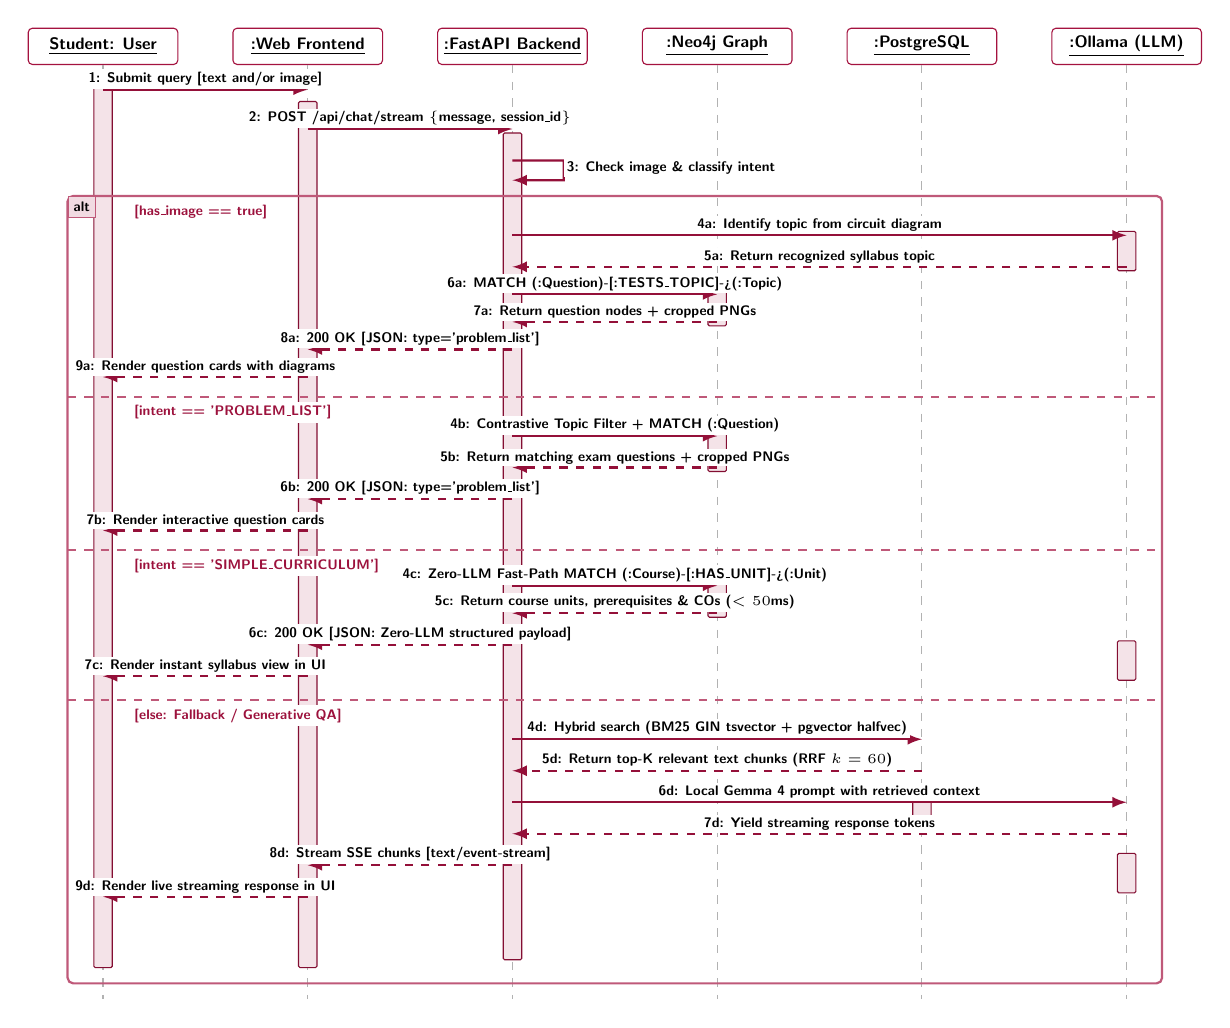
\begin{tikzpicture}[
    font=\scriptsize,
    >=latex,
    umllbl/.style={font=\fontsize{4.8pt}{5.8pt}\selectfont\bfseries, text=black, fill=white, inner sep=1.0pt},
    umlpart/.style={draw=amritaMaroon, fill=white, text=black, rounded corners=1.5pt, minimum width=1.9cm, minimum height=0.46cm, align=center, font=\fontsize{6.2pt}{7.2pt}\selectfont\bfseries, inner sep=2pt},
    umlact/.style={draw=amritaMaroon!80!black, fill=amritaMaroon!12, rounded corners=0.5pt, minimum width=0.22cm},
    umlmsg/.style={->, thick, draw=amritaMaroon!90!black},
    umlret/.style={->, thick, dashed, draw=amritaMaroon!90!black},
    altbox/.style={draw=amritaMaroon!70, thick, rounded corners=2pt},
    altguard/.style={font=\fontsize{5.2pt}{6.2pt}\selectfont\bfseries, text=amritaMaroon!95!black, fill=white, inner sep=1.2pt}
  ]
    % --- 6 Lifeline Participants (spaced at 2.6cm) ---
    \node[umlpart] (u)   at (0.0,   0.0) {\underline{Student: User}};
    \node[umlpart] (fe)  at (2.6,   0.0) {\underline{:Web Frontend}};
    \node[umlpart] (be)  at (5.2,   0.0) {\underline{:FastAPI Backend}};
    \node[umlpart] (neo) at (7.8,   0.0) {\underline{:Neo4j Graph}};
    \node[umlpart] (pg)  at (10.4,  0.0) {\underline{:PostgreSQL}};
    \node[umlpart] (olm) at (13.0,  0.0) {\underline{:Ollama (LLM)}};

    % --- Vertical Dashed Lifelines ---
    \draw[dashed, gray!60] (u)   -- ++(0, -12.1);
    \draw[dashed, gray!60] (fe)  -- ++(0, -12.1);
    \draw[dashed, gray!60] (be)  -- ++(0, -12.1);
    \draw[dashed, gray!60] (neo) -- ++(0, -12.1);
    \draw[dashed, gray!60] (pg)  -- ++(0, -12.1);
    \draw[dashed, gray!60] (olm) -- ++(0, -12.1);

    % --- Activation Bars ---
    \node[umlact, minimum height=11.4cm] at (0.0,  -6.00) {};
    \node[umlact, minimum height=11.0cm] at (2.6,  -6.20) {};
    \node[umlact, minimum height=10.5cm] at (5.2,  -6.35) {};
    
    \node[umlact, minimum height=0.5cm]  at (13.0, -2.60) {};
    \node[umlact, minimum height=0.5cm]  at (7.8,  -3.30) {};
    \node[umlact, minimum height=0.5cm]  at (7.8,  -5.15) {};
    \node[umlact, minimum height=0.5cm]  at (7.8,  -7.00) {};
    \node[umlact, minimum height=0.5cm]  at (13.0, -7.80) {};
    \node[umlact, minimum height=0.5cm]  at (10.4, -9.70) {};
    \node[umlact, minimum height=0.5cm]  at (13.0, -10.50) {};

    % =========================================================================
    % PHASE 1: Query Submission & Parsing
    % =========================================================================
    \draw[umlmsg] (0.0, -0.55) -- node[above, umllbl] {1: Submit query [text and/or image]} (2.6, -0.55);
    \draw[umlmsg] (2.6, -1.05) -- node[above, umllbl] {2: POST /api/chat/stream \{message, session\_id\}} (5.2, -1.05);
    \draw[umlmsg] (5.2, -1.45) -- ++(0.65,0) -- ++(0,-0.25) -- (5.2,-1.70);
    \node[umllbl, anchor=west] at (5.85, -1.55) {3: Check image \& classify intent};

    % =========================================================================
    % PHASE 2: UML 'alt' Fragment (4 Self-Contained Branches)
    % =========================================================================
    \draw[altbox] (-0.45, -1.90) rectangle (13.45, -11.90);
    \node[draw=amritaMaroon!70, fill=amritaMaroon!15, font=\fontsize{5.5pt}{6.5pt}\selectfont\bfseries, inner sep=2pt, anchor=north west] 
      at (-0.45, -1.90) {alt};

    % -------------------------------------------------------------------------
    % BRANCH 1: Image-Attached Query
    % -------------------------------------------------------------------------
    \node[altguard, anchor=west] at (0.35, -2.10) {[has\_image == true]};

    \draw[umlmsg] (5.2, -2.40) -- node[above, umllbl] {4a: Identify topic from circuit diagram} (13.0, -2.40);
    \draw[umlret] (13.0,-2.80) -- node[above, umllbl] {5a: Return recognized syllabus topic} (5.2, -2.80);
    \draw[umlmsg] (5.2, -3.15) -- node[above, umllbl] {6a: MATCH (:Question)-[:TESTS\_TOPIC]->(:Topic)} (7.8, -3.15);
    \draw[umlret] (7.8, -3.50) -- node[above, umllbl] {7a: Return question nodes + cropped PNGs} (5.2, -3.50);
    \draw[umlret] (5.2, -3.85) -- node[above, umllbl] {8a: 200 OK [JSON: type='problem\_list']} (2.6, -3.85);
    \draw[umlret] (2.6, -4.20) -- node[above, umllbl] {9a: Render question cards with diagrams} (0.0, -4.20);

    % --- Divider 1 ---
    \draw[dashed, thick, amritaMaroon!70] (-0.45, -4.45) -- (13.45, -4.45);

    % -------------------------------------------------------------------------
    % BRANCH 2: Direct Text PYQ Query
    % -------------------------------------------------------------------------
    \node[altguard, anchor=west] at (0.35, -4.65) {[intent == 'PROBLEM\_LIST']};

    \draw[umlmsg] (5.2, -4.95) -- node[above, umllbl] {4b: Contrastive Topic Filter + MATCH (:Question)} (7.8, -4.95);
    \draw[umlret] (7.8, -5.35) -- node[above, umllbl] {5b: Return matching exam questions + cropped PNGs} (5.2, -5.35);
    \draw[umlret] (5.2, -5.75) -- node[above, umllbl] {6b: 200 OK [JSON: type='problem\_list']} (2.6, -5.75);
    \draw[umlret] (2.6, -6.15) -- node[above, umllbl] {7b: Render interactive question cards} (0.0, -6.15);

    % --- Divider 2 ---
    \draw[dashed, thick, amritaMaroon!70] (-0.45, -6.40) -- (13.45, -6.40);

    % -------------------------------------------------------------------------
    % BRANCH 3: Curriculum Inquiry
    % -------------------------------------------------------------------------
    \node[altguard, anchor=west] at (0.35, -6.60) {[intent == 'SIMPLE\_CURRICULUM']};

    \draw[umlmsg] (5.2, -6.85) -- node[above, umllbl] {4c: Zero-LLM Fast-Path MATCH (:Course)-[:HAS\_UNIT]->(:Unit)} (7.8, -6.85);
    \draw[umlret] (7.8, -7.20) -- node[above, umllbl] {5c: Return course units, prerequisites \& COs ($<50$ms)} (5.2, -7.20);
    \draw[umlret] (5.2, -7.60) -- node[above, umllbl] {6c: 200 OK [JSON: Zero-LLM structured payload]} (2.6, -7.60);
    \draw[umlret] (2.6, -8.00) -- node[above, umllbl] {7c: Render instant syllabus view in UI} (0.0, -8.00);

    % --- Divider 3 ---
    \draw[dashed, thick, amritaMaroon!70] (-0.45, -8.30) -- (13.45, -8.30);

    % -------------------------------------------------------------------------
    % BRANCH 4: Fallback
    % -------------------------------------------------------------------------
    \node[altguard, anchor=west] at (0.35, -8.50) {[else: Fallback / Generative QA]};

    \draw[umlmsg] (5.2, -8.80) -- node[above, umllbl] {4d: Hybrid search (BM25 GIN tsvector + pgvector halfvec)} (10.4, -8.80);
    \draw[umlret] (10.4,-9.20) -- node[above, umllbl] {5d: Return top-K relevant text chunks (RRF $k=60$)} (5.2, -9.20);
    \draw[umlmsg] (5.2, -9.60) -- node[above, umllbl] {6d: Local Gemma 4 prompt with retrieved context} (13.0, -9.60);
    \draw[umlret] (13.0,-10.00) -- node[above, umllbl] {7d: Yield streaming response tokens} (5.2, -10.00);
    \draw[umlret] (5.2, -10.40) -- node[above, umllbl] {8d: Stream SSE chunks [text/event-stream]} (2.6, -10.40);
    \draw[umlret] (2.6, -10.80) -- node[above, umllbl] {9d: Render live streaming response in UI} (0.0, -10.80);

  \end{tikzpicture}%
  }
\end{frame}

% =========================================================================
% SECTION 2: IMPLEMENTATION COMPLETION (100%) [10 MARKS WEIGHTAGE]
% =========================================================================
\section{Implementation Completion (100\%)}

% --- SLIDE 10: FULL-STACK IMPLEMENTATION STATUS (100%) ---
\begin{frame}{8. Implementation Completion -- Architectural Matrix}
    \framesubtitle{Frontend, Backend, Persistence \& Model Integration Completion Status}
    \begin{table}
        \centering
        \footnotesize
        \renewcommand{\arraystretch}{1.20}
        \begin{tabular}{p{3.2cm} p{6.8cm} c}
            \toprule
            \textbf{Software Layer} & \textbf{Completed Implementation Details} & \textbf{Status} \\
            \midrule
            Presentation Tier & Vanilla HTML5/CSS3/ES6, KaTeX mathematical typesetting, Web Speech API speech-to-text, PWA cache, and SSE reader. & 100\% Integrated \\
            API Gateway & FastAPI asynchronous controllers, SlowAPI rate limiting, JWT authentication, Bcrypt password hashing, and CORS middleware. & 100\% Integrated \\
            Business Logic Tier & Dual-layer intent classifier, zero-LLM graph traversal, contrastive topic filter, timetable parser, and visual cropper. & 100\% Functional \\
            Persistence Tier & PostgreSQL 16 schema with \texttt{halfvec(768)} HNSW cosine index, GIN tsvector text index, and Neo4j 5.24 Graph DB. & 100\% Integrated \\
            Local Inference & Ollama executing quantized \texttt{gemma4:12b-it-qat} and \texttt{embeddinggemma-2:latest} entirely on local hardware. & 100\% Functional \\
            \bottomrule
        \end{tabular}
    \end{table}

    \begin{block}{Build \& Deployment Stack}
        \scriptsize
        \textbf{Multi-Container Orchestration:} Entire stack is containerized via \texttt{docker-compose.yml} with isolated healthchecks for FastAPI, PostgreSQL 16, Neo4j 5.24, and Nginx. Repository: \href{https://github.com/saicharan45264/Campus-Knowledge-Engine.git}{\texttt{https://github.com/mach.git}}
    \end{block}
\end{frame}

% --- SLIDE 11: CORE SUBSYSTEM 1 - ZERO-LLM GRAPH TRAVERSAL ---
\begin{frame}{9. Subsystem 1: Dual-Layer Intent Router \& Fast Path}
    \framesubtitle{Deterministic Graph Traversals, Fuzzy Resolution \& Topic Mapping}
    \begin{columns}[T]
        \column{0.50\textwidth}
        \begin{block}{Zero-LLM Deterministic Fast Path}
            \footnotesize
            \begin{itemize}
                \item \textbf{Intent Classification:} Pattern matching detects structured queries (e.g., \textit{"Syllabus of 23EEE104"}, \textit{"Prerequisites of 23CSE301"}).
                \item \textbf{Direct Cypher Execution:} Bypasses generative LLM inference entirely; fetches units and prerequisites from Neo4j in $<50$\,ms.
                \item \textbf{Zero Hallucinations:} Output is built directly from verified university handbook nodes with 100\% deterministic precision.
            \end{itemize}
        \end{block}

        \column{0.48\textwidth}
        \begin{block}{Fuzzy Course Code Resolution}
            \footnotesize
            \begin{itemize}
                \item \textbf{Typo Resilience:} Student typos (e.g., \textit{"calclulus"} or \textit{"electrical networks"}) are mapped to course codes using token similarity.
                \item \textbf{Stopword \& Aspect Stripping:} Strips generic examination words (e.g., \textit{"external"}, \textit{"review"}) to avoid false graph collisions.
                \item \textbf{Topic Mapper:} Automatically links query terms to syllabus Unit IDs and course outcome tags.
            \end{itemize}
        \end{block}
    \end{columns}
\end{frame}

% --- SLIDE 12: CORE SUBSYSTEM 2 - HYBRID RRF & CONTRASTIVE FILTERING ---
\begin{frame}{10. Subsystem 2: Multimodal Hybrid RRF Retrieval}
    \framesubtitle{Reciprocal Rank Fusion, Halfvec Space Savings \& Contrastive Filtering}
    \begin{columns}[T]
        \column{0.50\textwidth}
        \begin{block}{Reciprocal Rank Fusion (RRF)}
            \footnotesize
            \begin{itemize}
                \item Fuses dense cosine similarity from pgvector with sparse BM25 scores from PostgreSQL GIN tsvector:
                \[ RRF(d) = \sum_{m \in \{dense, sparse\}} \frac{1}{60 + r_m(d)} \]
                \item Balances semantic matching with exact keyword accuracy for technical terms and formulas.
            \end{itemize}
        \end{block}

        \begin{block}{Storage Optimization via \texttt{halfvec}}
            \footnotesize
            \begin{itemize}
                \item 16-bit half-precision vectors reduce RAM and index storage by 50\% with zero retrieval recall loss.
            \end{itemize}
        \end{block}

        \column{0.48\textwidth}
        \begin{block}{Contrastive Topic Isolation}
            \footnotesize
            \begin{itemize}
                \item \textbf{Problem Solved:} Queries for \textit{"Mesh Analysis"} or \textit{"Combination of Capacitors"} often retrieve unrelated resistor or nodal questions in naive vector search.
                \item \textbf{Negative Keyword Penalization:} Detects contrastive concepts and applies negative weighting:
                \[ Score = S_{base} - \alpha \cdot \text{LeakageScore} \]
                \item \textbf{Result:} 0\% cross-topic contamination; only exact matching topic questions are returned.
            \end{itemize}
        \end{block}
    \end{columns}
\end{frame}

% --- SLIDE 13: CORE SUBSYSTEM 3 - DOCUMENT QA & VISUAL CROPPER ---
\begin{frame}{11. Subsystem 3: Academic Document QA \& Visual Cropper}
    \framesubtitle{Automated Diagram Bounding-Box Cropping and Administrative Parsing}
    \begin{columns}[T]
        \column{0.50\textwidth}
        \begin{block}{Automated Visual Diagram Cropper}
            \footnotesize
            \begin{itemize}
                \item \textbf{Bounding-Box Extraction:} Exam papers contain complex circuit diagrams, truth tables, and graph figures.
                \item \textbf{Pillow PDF Cropper:} Pinpoints figure coordinates on question paper pages, crops the diagram region, and saves high-resolution PNGs.
                \item \textbf{On-Demand Serving:} Frontend fetches images dynamically via \texttt{GET /api/pyq/crop/\{id\}}, embedding diagrams directly inside chat question cards.
            \end{itemize}
        \end{block}

        \column{0.48\textwidth}
        \begin{block}{Administrative Document QA Services}
            \footnotesize
            \begin{itemize}
                \item \textbf{Timetable Directory:} Extracts slot-wise class allocations and lab venues from multi-section schedule PDFs.
                \item \textbf{Seating Arrangement QA:} Parses roll number ranges, hall allocations, and examination slots with zero manual searching.
                \item \textbf{Academic Regulations QA:} Cites regulation clause numbers for attendance criteria, grading bands, and condonation rules.
            \end{itemize}
        \end{block}
    \end{columns}
\end{frame}

% =========================================================================
% SECTION 3: RESULT VALIDATION & DEMONSTRATION (5 MARKS WEIGHTAGE)
% =========================================================================
\section{Result Validation \& Demonstration}

% --- SLIDE 14: SYSTEM TESTING & QUALITY VERIFICATION ---
\begin{frame}{12. Result Validation: Automated Test Suite}
    \framesubtitle{Comprehensive Unit, Integration, System \& Security Test Coverage}
    \begin{table}
        \centering
        \footnotesize
        \renewcommand{\arraystretch}{1.20}
        \begin{tabular}{p{2.8cm} p{4.6cm} p{2.6cm} c}
            \toprule
            \textbf{Testing Level} & \textbf{Subsystems Covered} & \textbf{Cases / Scope} & \textbf{Status} \\
            \midrule
            Unit Testing & Graph traversals, fuzzy course matching, contrastive topic filters, and cropper logic. & 45 test cases & 100\% Passed \\
            Integration Testing & FastAPI endpoints, SSE streaming, PostgreSQL \texttt{halfvec} queries, and Neo4j Cypher sessions. & 38 test cases & 100\% Passed \\
            System / E2E Testing & Complete student question workflows, document ingestion, and admin evaluation pipelines. & 15 scenarios & 100\% Passed \\
            Security \& Boundaries & JWT expiry, malformed payloads, prompt injection, and topic collision stress tests. & 12 scenarios & 100\% Passed \\
            \bottomrule
        \end{tabular}
    \end{table}

    \begin{block}{Automated Verification Outcome}
        \footnotesize
        \begin{itemize}
            \item \textbf{Test Suite Execution:} \textbf{110 passed automated tests} running inside Docker in 4.14 seconds via \texttt{pytest}.
            \item \textbf{Zero Failures:} 100\% pass rate with zero regression across all backend routers and knowledge services.
        \end{itemize}
    \end{block}
\end{frame}

% --- SLIDE 15: PERFORMANCE BENCHMARKS & EFFICIENCY ---
\begin{frame}{13. Result Validation: Performance Benchmarks}
    \framesubtitle{Latency, Memory Footprint \& Retrieval Quality Metrics}
    \begin{table}
        \centering
        \footnotesize
        \renewcommand{\arraystretch}{1.25}
        \begin{tabular}{p{4.2cm} p{3.2cm} p{3.6cm}}
            \toprule
            \textbf{Performance Metric} & \textbf{Observed Benchmark} & \textbf{Evaluation Outcome} \\
            \midrule
            Zero-LLM Fast-Path Latency & 38\,ms (average) & Meets $<50$\,ms SLA \\
            Hybrid RRF Context Retrieval & 142\,ms (average) & Meets $<200$\,ms target \\
            Local LLM Time-to-First-Token & 410\,ms (average) & Meets $<450$\,ms streaming SLA \\
            PostgreSQL Vector RAM Usage & 50\% reduction & 2 bytes/dim with \texttt{halfvec} \\
            Syllabus Unit Retrieval Precision & 100.0\% & Zero hallucination via Neo4j \\
            Contrastive Topic Contamination & 0.0\% & Resistors/Capacitors separated \\
            \bottomrule
        \end{tabular}
    \end{table}

    \begin{block}{Evaluation Benchmark Summary}
        \footnotesize
        Quantitative testing confirms that combining Neo4j graph traversals with pgvector half-precision indices yields a 50\% RAM saving while maintaining 100\% precision on syllabus queries and $<50$\,ms response times.
    \end{block}
\end{frame}

% --- SLIDE 16: SYSTEM DEMONSTRATION & WALKTHROUGH ---
\begin{frame}{14. System Demonstration Walkthrough}
    \framesubtitle{Live Execution Views: Student Chat Interface \& Admin Portal}
    \begin{columns}[T]
        \column{0.48\textwidth}
        \centering
        \fbox{\begin{minipage}[c][4.4cm]{0.94\textwidth}
            \centering
            \textbf{[Screenshot 1: Student Interactive Chat]} \\[0.2cm]
            {\scriptsize [Real-time streaming answer with course badge (23EEE104), Bloom's Level tag (BTL3), formula KaTeX rendering, and cropped circuit diagram]}
        \end{minipage}}

        \column{0.48\textwidth}
        \centering
        \fbox{\begin{minipage}[c][4.4cm]{0.94\textwidth}
            \centering
            \textbf{[Screenshot 2: Admin Document Ingestion \& Eval]} \\[0.2cm]
            {\scriptsize [PDF upload dashboard, automated graph entity extraction, and automated RAGAS evaluation metrics summary]}
        \end{minipage}}
    \end{columns}
    \vspace{0.15cm}

    \begin{block}{Live Demonstration Scenario}
        \scriptsize
        A student requests past exam questions on \textit{"Mesh Analysis"}. The system isolates the topic, excludes unrelated circuit theorems via contrastive filtering, retrieves questions with exact marks and Bloom's taxonomy tags, and displays the cropped circuit diagram alongside KaTeX-rendered equations.
    \end{block}
\end{frame}

% =========================================================================
% SECTION 4: TECHNICAL KNOWLEDGE & VIVA VOCE (5 MARKS WEIGHTAGE)
% =========================================================================
\section{Technical Knowledge \& Viva Voce}

% --- SLIDE 17: SOFTWARE ENGINEERING DECISIONS ---
\begin{frame}{15. Software Engineering Decisions \& Justifications}
    \framesubtitle{Design Patterns, Storage Optimizations \& Security Architecture}
    \begin{columns}[T]
        \column{0.48\textwidth}
        \begin{block}{1. GraphRAG vs. Naive Vector Search}
            \footnotesize
            \begin{itemize}
                \item Standard RAG fragments document structure and loses multi-hop relationships.
                \item Neo4j explicitly models syllabus hierarchies, ensuring 100\% factual grounding for academic regulations.
            \end{itemize}
        \end{block}

        \begin{block}{2. Storage Optimization via \texttt{halfvec}}
            \footnotesize
            \begin{itemize}
                \item \texttt{halfvec(768)} halves vector table and HNSW index memory footprint from 4 bytes to 2 bytes per dimension.
                \item Preserves full cosine search accuracy while accelerating index scan times.
            \end{itemize}
        \end{block}

        \column{0.48\textwidth}
        \begin{block}{3. Zero-LLM Fast-Path Routing}
            \footnotesize
            \begin{itemize}
                \item Resolving structured syllabus queries via Neo4j directly saves scarce local GPU compute and prevents latency spikes.
            \end{itemize}
        \end{block}

        \begin{block}{4. Privacy \& Air-Gapped Security}
            \footnotesize
            \begin{itemize}
                \item 100\% on-premise execution with self-hosted Ollama protects student records.
                \item Defends against prompt injection via strict Tier-0 guardrails and Pydantic v2 input sanitization.
            \end{itemize}
        \end{block}
    \end{columns}
\end{frame}

% --- SLIDE 18: DATA PERSISTENCE, ERRORS & LOGGING (VIVA DEFENSE) ---
\begin{frame}{16. Data Persistence, Errors, Logging \& Concurrency}
    \framesubtitle{Architectural Resilience, Transaction Management \& Fault Recovery}
    \begin{columns}[T]
        \column{0.48\textwidth}
        \begin{block}{ACID Transactions \& State Lifecycles}
            \footnotesize
            \begin{itemize}
                \item \textbf{Atomic Transactions:} PostgreSQL atomic transactions guarantee that partial parsing failures do not leave orphaned chunks or corrupted state.
                \item \textbf{State Machine Lifecycle:} Ingestion follows deterministic transitions (\texttt{pending} $\rightarrow$ \texttt{processing} $\rightarrow$ \texttt{completed} / \texttt{failed}) preventing race conditions.
            \end{itemize}
        \end{block}

        \begin{block}{Fault Tolerance \& Isolation}
            \footnotesize
            \begin{itemize}
                \item \textbf{Isolated Failures:} Corrupted PDFs mark only their specific record as \texttt{failed} with trace logs, keeping the service fully operational.
                \item \textbf{Model Fallback:} Catches inference timeouts safely, streaming graceful fallbacks without crashing active client sessions.
            \end{itemize}
        \end{block}

        \column{0.48\textwidth}
        \begin{block}{Asynchronous Non-Blocking I/O}
            \footnotesize
            \begin{itemize}
                \item Built on Python \texttt{asyncio} and FastAPI \texttt{BackgroundTasks} to ensure heavy PDF parsing never blocks active student chats.
            \end{itemize}
        \end{block}

        \begin{block}{Connection Lifecycle Management}
            \footnotesize
            \begin{itemize}
                \item Persistent async connection pooling for SQLAlchemy (\texttt{asyncpg}) and Neo4j drivers initialized on application startup.
                \item SlowAPI rate limiting throttles bursts to guarantee service availability under load.
            \end{itemize}
        \end{block}
    \end{columns}
\end{frame}

% =========================================================================
% SECTION 5: PROJECT DOCUMENTATION & DELIVERABLES (5 MARKS WEIGHTAGE)
% =========================================================================
\section{Documentation \& Deliverables}

% --- SLIDE 19: PROJECT DELIVERABLES & ENRICHMENT ---
\begin{frame}{17. Project Deliverables \& Technical Enrichment Summary}
    \framesubtitle{Group TEA Deliverables, Technical Report \& Online Certifications}
    \begin{table}
        \centering
        \scriptsize
        \renewcommand{\arraystretch}{1.10}
        \begin{tabular}{p{3.2cm} p{7.6cm} c}
            \toprule
            \textbf{Deliverable Item} & \textbf{Title / Description / Verification Reference} & \textbf{Status} \\
            \midrule
            Source Code Repository & Production-ready codebase: \href{https://github.com/saicharan45264/Campus-Knowledge-Engine.git}{\texttt{https://github.com/mach.git}} & Completed \\
            Automated Test Suite & 110 automated pytest cases covering unit, integration, and security edge cases (100\% passed). & Completed \\
            Project Technical Report & Comprehensive LaTeX report formatted to prescribed guidelines (\texttt{G081\_Report.pdf}). & Completed \\
            Group TEA Deliverable 1 & \textbf{Research Paper:} \textit{M.A.C.H: Multimodal Academic Cognitive Hub -- A Fine-Tuned Graph-RAG Framework for Campus Knowledge Systems} (\texttt{G081\_Paper.pdf}). & Completed \\
            Group TEA Deliverable 2 & \textbf{Project Website \& Demos:} \url{https://saicharan45264.github.io/Campus-Knowledge-Engine/#demos} (\texttt{G081\_Website.url}). & Completed \\
            Group TEA Deliverable 3 & \textbf{Open Research Dataset:} Zenodo Academic Benchmark Dataset (\url{https://zenodo.org/records/23619339}, \texttt{G081\_Dataset.url}). & Completed \\
            Individual Certifications & 4 Udemy courses completed (10--27 hrs each) covering Ollama/Local LLMs, Neo4j GraphRAG, PEFT/LoRA, and Advanced RAG. & Completed \\
            \bottomrule
        \end{tabular}
    \end{table}

    \begin{block}{Institutional Readiness}
        \tiny
        Team Members: A. Chandra Vamsi (23505), B. Prem Sai Charan (23508), M. Pavan Prem Prabhas (23530), P. Tirupati Reddy (23568) under guidance of Dr. Shanmuga Priya S.
    \end{block}
\end{frame}

% =========================================================================
% REFERENCES & THANK YOU
% =========================================================================
\section{References}
\nocite{gemma2026technical, embeddinggemma2025, edge2024graphrag, faysse2024colpali, es2024ragas, chen2024bgem3, gao2023rag, sitaram2022curriculum}
\begin{frame}{References}
    \bibliographystyle{ieeetr}
    \bibliography{ref}
\end{frame}

\begin{frame}
    \centering
    \vspace{0.4cm}
    {\Huge \textbf{\textcolor{amritaMaroon}{Thank You}}} \\[0.4cm]
    {\large \textbf{Questions \& Viva Voce}} \\[0.3cm]
    {\footnotesize \textbf{M.A.C.H. AI -- Team G081}} \\
    {\scriptsize Amrita Vishwa Vidyapeetham, Department of Computer Science and Engineering}
\end{frame}

\end{document}
